% homework/hw03/hw03.tex
% Year 7 - Homework Packet 3
% Covers Maths 1.4 (highest common factors), Maths 1.5 (tests for
% divisibility) and Science 1.4 (cells, tissues and organs).
%
% Division practice is built into the maths on purpose, and it is motivated
% rather than bolted on: A2 divides to decide whether a number is a factor,
% A4 divides top and bottom by the HCF, and B2 makes the class prove the
% divisibility tests they ticked in B1 by actually carrying out the division.
% That is roughly thirty divisions across the packet without a single naked
% "do these sums" block.
%
% House style is shared: see homework/hw-style.tex. Method: the new-homework
% skill. Source is pure ASCII on purpose.
%
% Build:  pwsh .claude/skills/new-homework/scripts/build-hw.ps1 hw03

\documentclass[12pt,a4paper]{article}

% -- Answer key switch -------------------------------------------------------
\newif\ifkey
\ifdefined\TEACHER\keytrue\else
  \keyfalse        % \keyfalse = student copy   |   \keytrue = teacher copy
\fi

% -- House style -------------------------------------------------------------
% homework/hw-style.tex
% Shared house style for every Year 7 homework packet. \input this from the
% packet file, right after \documentclass and the answer-key switch.
%
% Do not fork this file per packet. If a packet needs a different look, the
% question is whether every packet should have it.
%
% The choices here are deliberate and were arrived at by printing and looking:
%   * No solid dark banners. Every header is a light tint with a coloured spine
%     on the left, so colour reads clearly without flooding a school printer.
%   * No marks and no mark totals. These are practice, not exam papers.
%   * Lato at 12pt with open leading, plus mathastext so inline maths is Lato
%     too. Without mathastext every "-6 + 4" is Computer Modern serif and the
%     sheet looks half-typeset.
%   * Writing lines are spaced for Year 7 handwriting, not adult margin notes.
%
% Provides: \wlines \blank \tickbox \sep \qmk-free marks (none) \hwsection
% \qhead \expr, the workspace box, and the remember / wordhelp / activity /
% yourturn coloured boxes. Palette matches the lesson decks exactly.

% -- Packages ----------------------------------------------------------------
\usepackage[T1]{fontenc}
\usepackage[utf8]{inputenc}
\usepackage[default]{lato}
\usepackage[a4paper,top=1.7cm,bottom=1.7cm,left=2.0cm,right=2.0cm,headheight=15pt]{geometry}
\usepackage{amsmath,amssymb}
\usepackage{xcolor}
\usepackage[most]{tcolorbox}
\usepackage{enumitem}
\usepackage{tikz}
\usetikzlibrary{arrows.meta}
\usepackage{array}
\usepackage{tabularx}
\usepackage{fancyhdr}
\usepackage{multicol}
\usepackage{needspace}
\usepackage{graphicx}

% Make maths use Lato too. Without this, every "-6 + 4" on the page is set in
% Computer Modern serif and the sheet looks half-typeset. Must come last.
\usepackage[italic]{mathastext}

\linespread{1.06}\selectfont

% -- The Learner's Book palette (same hex values as the lesson decks) ---------
\definecolor{cbteal}{HTML}{0087A8}
\definecolor{cbpurple}{HTML}{5C2483}
\definecolor{cborange}{HTML}{C25E12}
\definecolor{cbgreen}{HTML}{4A8B23}
\definecolor{cbred}{HTML}{C8102E}
\definecolor{cbblue}{HTML}{1A5FA8}
\definecolor{rulegray}{HTML}{9AA5AD}

% -- Answer lines and blanks -------------------------------------------------
% \wlines{n} draws n ruled writing lines, spaced wide enough for Year 7
% handwriting rather than for an adult with a fine pen.
\makeatletter
\newcommand{\wlines}[1]{%
  \par\vspace{0.75em}%
  \@tempcnta=0\relax
  \@whilenum\@tempcnta<#1\do{%
    \hbox to \linewidth{\color{rulegray}\leaders\hrule height 0.5pt\hfill}%
    \vspace{1.5em}%
    \advance\@tempcnta by 1\relax}%
  \par\vspace{-0.8em}%
}
\makeatother

% \blank[width] is an inline gap to write a short answer in.
\newcommand{\blank}[1][2.6cm]{\underline{\hspace{#1}}}

% A boxed space for showing working.
\newtcolorbox{workspace}[1][3.4cm]{%
  colback=white, colframe=rulegray, boxrule=0.5pt, arc=5pt,
  height=#1, left=6pt, right=6pt, top=4pt, bottom=4pt,
  before skip=9pt, after skip=11pt}

% An empty tick box.
\newcommand{\tickbox}{\fbox{\rule{0pt}{1.15em}\rule{1.15em}{0pt}}}

% A middot separator.
\newcommand{\sep}{\,\textperiodcentered\,}

% -- Section and question headings -------------------------------------------
% Light tint plus a fat coloured spine on the left. No solid dark banner: the
% colour reads clearly but barely costs the printer anything.
% needspace stops a heading stranding alone at the foot of a page. Kept modest:
% too large and it pushes headings over, leaving a worse hole than it prevents.
\newcommand{\hwsection}[2][cbteal]{%
  \needspace{8\baselineskip}%
  \par\vspace{13pt}%
  \noindent
  \begin{tcolorbox}[enhanced, nobeforeafter, width=\textwidth,
      colback=#1!7, colframe=#1!7, arc=5pt,
      borderline west={5pt}{0pt}{#1},
      left=14pt, right=10pt, top=7pt, bottom=7pt]
    {\large\bfseries\color{#1}#2}
  \end{tcolorbox}%
  \par\vspace{9pt}}

% \qhead[colour]{A2}{Moving along the line} -- a question heading.
\newcommand{\qhead}[3][cbteal]{%
  \needspace{6\baselineskip}%
  \par\vspace{11pt}%
  \noindent{\large\bfseries\color{#1}#2}\quad{\large\bfseries #3}\par\vspace{4pt}}

% -- Coloured boxes ----------------------------------------------------------
% Shared look: rounded, light fill, coloured rule, coloured title text on a
% pale title strip rather than a dark one.
\tcbset{hwbox/.style={
  enhanced, breakable, arc=6pt, boxrule=1pt,
  left=11pt, right=11pt, top=8pt, bottom=8pt,
  fonttitle=\bfseries, attach boxed title to top left={xshift=12pt, yshift=-8pt},
  boxed title style={arc=4pt, boxrule=1pt, left=7pt, right=7pt, top=2pt, bottom=2pt},
  top=13pt}}

% Orange: things to remember. Matches the deck's "Write This Down".
\newtcolorbox{remember}[1][Remember from the lesson]{hwbox,
  colback=cborange!6, colframe=cborange, coltitle=cborange,
  colbacktitle=white, title={#1}}

% Blue: English help. The barrier in this class is the wording, not the maths.
\newtcolorbox{wordhelp}[1][Word help]{hwbox,
  colback=cbblue!6, colframe=cbblue, coltitle=cbblue,
  colbacktitle=white, title={#1}}

% Purple: an activity or instruction.
\newtcolorbox{activity}[1][How to do this homework]{hwbox,
  colback=cbpurple!6, colframe=cbpurple, coltitle=cbpurple,
  colbacktitle=white, title={#1}}

% Green: your turn / a friendly nudge.
\newtcolorbox{yourturn}[1][Your turn]{hwbox,
  colback=cbgreen!7, colframe=cbgreen, coltitle=cbgreen!75!black,
  colbacktitle=white, title={#1}}

% -- Shorthands --------------------------------------------------------------
\newcommand{\dC}{\,^{\circ}\mathrm{C}}          % use inside maths: $-8\dC$
\newcommand{\key}[1]{{\color{cborange}\textbf{#1}}}
\newcommand{\eng}[1]{{\color{cbblue}\textbf{#1}}}

\setlist[enumerate]{itemsep=8pt, topsep=5pt, leftmargin=*}
\setlist[itemize]{itemsep=4pt, topsep=4pt, leftmargin=*}
\renewcommand{\arraystretch}{1.45}

% -- An expression the student is asked to work from -------------------------
\newcommand{\expr}[1]{%
  \tcbox[on line, colback=cbgreen!10, colframe=cbgreen!55, boxrule=1pt, arc=4pt,
         left=9pt, right=9pt, top=4pt, bottom=4pt]{\large\bfseries $#1$}}

% -- Running head and foot ---------------------------------------------------
% The packet overrides \fancyhead[L] with its own title.
\pagestyle{fancy}
\fancyhf{}
\fancyhead[L]{\small\color{black!55}Year 7\sep Homework}
\fancyhead[R]{\small\color{black!55}Name: \blank[3.4cm]}
\fancyfoot[C]{\small\color{black!55}Page \thepage}
\renewcommand{\headrulewidth}{0pt}
\renewcommand{\headrule}{\vspace{2pt}\hbox to\headwidth{\color{cbteal!45}\leaders\hrule height 1.2pt\hfill}}



% -- Per-packet running head -------------------------------------------------
\fancyhead[L]{\small\color{black!55}Year 7\sep Homework 3}

\begin{document}

% ===========================================================================
% COVER BLOCK
% ===========================================================================
\thispagestyle{fancy}

\begin{tcolorbox}[enhanced, colback=cbpurple!7, colframe=cbpurple!7, arc=7pt,
                  borderline west={6pt}{0pt}{cbpurple},
                  left=18pt, right=14pt, top=14pt, bottom=14pt]
  {\color{cbpurple}\bfseries YEAR 7\sep UNIT 1\sep HOMEWORK 3}\\[6pt]
  {\color{cbpurple}\Huge\bfseries Factors, Tests and Tissues}\\[10pt]
  {\color{black!70}Mathematics 1.4 --- Highest Common Factors\sep
   1.5 --- Tests for Divisibility}\\
  {\color{black!70}Science 1.4 --- Cells, Tissues and Organs}
\end{tcolorbox}

\vspace{10pt}
\noindent
\begin{tabularx}{\textwidth}{@{}X X@{}}
  \textbf{Name:} \blank[5.6cm] & \textbf{Class:} \blank[5.6cm] \\
  \textbf{Date given:} \blank[4.6cm] & \textbf{Date due:} \blank[5.0cm] \\
\end{tabularx}

\vspace{8pt}
\begin{activity}
  \begin{itemize}
    \item Write your answers \textbf{on this sheet}, in the spaces given. If you need
          more room, use the back of the page.
    \item In maths, \key{write the division, not just the answer}. Almost every
          question in Section A and Section B is really a division question.
    \item In science, answer in \key{full English sentences}. ``Organ'' is not a
          sentence; ``The heart is an organ'' is. If a word is new to you, look for the
          blue \eng{Word help} box on that page before you give up.
  \end{itemize}
\end{activity}

% ===========================================================================
% SECTION A -- MATHS 1.4
% ===========================================================================
\hwsection{Section A \textperiodcentered\ Mathematics 1.4 --- Highest Common Factors}

\begin{remember}
  A \key{factor} of a number divides into it \key{exactly}, with nothing left over.
  You find factors by hunting for \key{pairs}: $24 = 1 \times 24$, $2 \times 12$,
  $3 \times 8$, $4 \times 6$.

  \medskip
  \key{Common} means \key{shared}. A \key{common factor} is in both lists, and the
  \key{highest common factor (HCF)} is the biggest of them --- the same idea you
  already know as \key{UCLN}.

  \medskip
  \key{The HCF is never ``none''.} 1 is a factor of every number, so every pair has
  at least one common factor.
\end{remember}

% -- A1 ---------------------------------------------------------------------
\qhead{A1}{Hunt the pairs}

\noindent\textbf{(a)} Write \textbf{every} pair of whole numbers that multiplies to
\textbf{36}, then list all the factors of 36.

\vspace{4pt}
\noindent\hspace*{1em}Pairs: \blank[12.4cm]

\vspace{6pt}
\noindent\hspace*{1em}Factors of 36: \blank[11.2cm]

\vspace{9pt}
\noindent\textbf{(b)} Now do the same for \textbf{54}.

\vspace{4pt}
\noindent\hspace*{1em}Pairs: \blank[12.4cm]

\vspace{6pt}
\noindent\hspace*{1em}Factors of 54: \blank[11.2cm]

\vspace{9pt}
\noindent\textbf{(c)} Which numbers are in \textbf{both} lists? \blank[9.4cm]

\vspace{8pt}
\noindent\textbf{(d)} So the \textbf{HCF} of 36 and 54 is \blank[3cm]

% -- A2 ---------------------------------------------------------------------
\qhead{A2}{Divide to decide}

\begin{remember}[The only way to be sure]
  There is one test that always works: \key{do the division}. If there is
  \key{nothing left over}, it is a factor. If there is a \key{remainder}, it is not.
\end{remember}

\noindent Do each division. Write the answer, and the remainder if there is one. Then
tick the box only if the first number is a \textbf{factor}.

\vspace{10pt}
% The Division columns are fixed width, not X. As X columns they took whatever
% was left after the answer boxes and "156 div 12" wrapped onto two lines.
\noindent
\begin{tabularx}{\textwidth}{|p{2.2cm}|X|c|p{2.2cm}|X|c|}
  \hline
  \textbf{Division} & \textbf{Answer} & \textbf{Factor?} &
  \textbf{Division} & \textbf{Answer} & \textbf{Factor?} \\
  \hline
  $96 \div 6$  \rule[-0.8em]{0pt}{2.15em} & & \tickbox & $96 \div 7$  & & \tickbox \\ \hline
  $84 \div 4$  \rule[-0.8em]{0pt}{2.15em} & & \tickbox & $84 \div 5$  & & \tickbox \\ \hline
  $105 \div 7$ \rule[-0.8em]{0pt}{2.15em} & & \tickbox & $132 \div 8$ & & \tickbox \\ \hline
  $156 \div 12$\rule[-0.8em]{0pt}{2.15em} & & \tickbox & $210 \div 6$ & & \tickbox \\ \hline
\end{tabularx}

% -- A3 ---------------------------------------------------------------------
\qhead{A3}{Say it, then write it}

\begin{wordhelp}[Word help --- the English tells you which number to start with]
  \begin{tabularx}{\linewidth}{@{}lX@{}}
    \eng{divide 96 by 8}          & you \textbf{start} at 96: $96 \div 8$. \\
    \eng{share 72 equally between 9} & divide: $72 \div 9$. \\
    \eng{6 divides into 84}       & $84 \div 6$, not $6 \div 84$. \\
    \eng{exactly}                 & with \textbf{nothing left over}. No remainder. \\
    \eng{the highest common factor of} & the \textbf{biggest} number that divides into
                                    \textbf{both}. \\
    \eng{in its simplest form}    & written with the \textbf{smallest} numbers you can. \\
  \end{tabularx}
\end{wordhelp}

\noindent Turn each sentence into a calculation, then work it out.
\key{Write the calculation first.}

\vspace{6pt}
\begin{enumerate}[label=\arabic*., itemsep=8pt]
  \item Divide 96 by 8. \\[4pt]
        Calculation: \blank[6.2cm] \quad Answer: \blank[2.4cm]
  \item Share 72 equally between 9. \\[4pt]
        Calculation: \blank[6.2cm] \quad Answer: \blank[2.4cm]
  \item Find the highest common factor of 20 and 30. \\[4pt]
        Calculation: \blank[6.2cm] \quad Answer: \blank[2.4cm]
  \item Does 6 divide into 81 exactly? Show the division. \\[4pt]
        Calculation: \blank[6.2cm] \quad Answer: \blank[2.4cm]
\end{enumerate}

% -- A4 ---------------------------------------------------------------------
\qhead{A4}{What the HCF is actually for}

\begin{remember}[Simplest form in one step]
  Find the HCF of the top and the bottom, then \key{divide both of them by it}.
  That is the whole method --- and it is two more divisions.
\end{remember}

\noindent Write each fraction in its simplest form. Fill in every box.

\vspace{10pt}
\noindent
\begin{tabularx}{\textwidth}{|c|p{2.2cm}|X|X|p{2.4cm}|}
  \hline
  \textbf{Fraction} & \textbf{HCF} & \textbf{Top $\div$ HCF} & \textbf{Bottom $\div$ HCF}
  & \textbf{Simplest form} \\
  \hline
  $\dfrac{18}{24}$ \rule[-1.2em]{0pt}{3.0em} & & & & \\ \hline
  $\dfrac{30}{45}$ \rule[-1.2em]{0pt}{3.0em} & & & & \\ \hline
  $\dfrac{48}{60}$ \rule[-1.2em]{0pt}{3.0em} & & & & \\ \hline
\end{tabularx}

% -- A5 ---------------------------------------------------------------------
\qhead[cbgreen]{A5}{Two answers that surprise people}

\begin{yourturn}[Work these out before you read on]
  Both of these pairs catch nearly everybody. Do the factor lists if you need to.
\end{yourturn}

\noindent\textbf{(a)} The HCF of \textbf{9 and 10} is \blank[3cm]

\vspace{6pt}
\noindent\textbf{(b)} The HCF of \textbf{7 and 42} is \blank[3cm]

\vspace{8pt}
\noindent\textbf{(c)} A student writes that 9 and 10 have \textbf{no} common factor.
In one full sentence, explain why that can never be true for any pair of numbers.
\wlines{2}

% -- A6 ---------------------------------------------------------------------
\qhead{A6}{Word problems}

\noindent Read each one \key{all the way to the end} before you start writing.

\begin{enumerate}[label=\textbf{\arabic*.}, itemsep=14pt]

  \item \textbf{The bracelets.} Mr Bowen has \textbf{42 red beads} and
        \textbf{56 blue beads}. He makes identical bracelets from them, using every
        bead, with \textbf{nothing left over}, and he wants \textbf{as many
        bracelets as possible}. How many bracelets can he make, and how many beads
        of each colour go on one bracelet?
        \begin{workspace}[2.7cm]\end{workspace}

  \item \textbf{The test.} There are \textbf{60 questions} on a test. Mr Bowen gets
        \textbf{45} of them right. Write the fraction he got right, in its
        \textbf{simplest form}.
        \begin{workspace}[2.4cm]\end{workspace}

\end{enumerate}

% ===========================================================================
% SECTION B -- MATHS 1.5
% ===========================================================================
\hwsection{Section B \textperiodcentered\ Mathematics 1.5 --- Tests for Divisibility}

% Two things here are deliberate. The label column is `l`, not `p{}`: as a
% p-column every label printed half a line BELOW its own description. And the
% row stretch is cut locally, because at the global 1.45 this nine-row box was
% tall enough to be pushed to the next page, stranding the section heading
% alone at the foot of the previous one.
\begin{remember}[The nine tests you wrote down]
  {\renewcommand{\arraystretch}{1.12}%
  \begin{tabularx}{\linewidth}{@{}l@{\hspace{1.4em}}X@{}}
    \key{by 2}  & the last digit is 0, 2, 4, 6 or 8 \\
    \key{by 3}  & the digits add up to a multiple of 3 \\
    \key{by 4}  & the last \textbf{two} digits make a multiple of 4 \\
    \key{by 5}  & the last digit is 0 or 5 \\
    \key{by 6}  & it passes the test for 2 \textbf{and} the test for 3 \\
    \key{by 8}  & the last \textbf{three} digits make a multiple of 8 \\
    \key{by 9}  & the digits add up to a multiple of 9 \\
    \key{by 10} & the last digit is 0 \\
    \key{by 11} & split the digits into two groups, taking every other one, and add
                  each group. The \textbf{difference} is 0 or a multiple of 11 \\
  \end{tabularx}}

  \smallskip
  There is \key{no easy test for 7}. For 7 you divide and look at the remainder.
\end{remember}

% -- B1 ---------------------------------------------------------------------
\qhead{B1}{The factor hunt}

\noindent Use the tests. Put a \textbf{tick} in the box if the number on the left
divides by the number at the top, and a \textbf{cross} if it does not. Do \textbf{not}
use a calculator.

\vspace{10pt}
% Fixed label column, X for the nine tick columns: with the label column as X
% it swallowed the width and left nine boxes too small to tick.
\noindent
\begin{tabularx}{\textwidth}{|p{2.3cm}|*{9}{>{\centering\arraybackslash}X|}}
  \hline
  & \textbf{2} & \textbf{3} & \textbf{4} & \textbf{5} & \textbf{6} & \textbf{8}
  & \textbf{9} & \textbf{10} & \textbf{11} \\
  \hline
  \textbf{1260} \rule[-0.9em]{0pt}{2.45em} & & & & & & & & & \\ \hline
  \textbf{3465} \rule[-0.9em]{0pt}{2.45em} & & & & & & & & & \\ \hline
  \textbf{2088} \rule[-0.9em]{0pt}{2.45em} & & & & & & & & & \\ \hline
  \textbf{4510} \rule[-0.9em]{0pt}{2.45em} & & & & & & & & & \\ \hline
  \textbf{5832} \rule[-0.9em]{0pt}{2.45em} & & & & & & & & & \\ \hline
\end{tabularx}

\vspace{10pt}
\noindent Now pick \textbf{one} of your ticks and say which test proved it.

\vspace{4pt}
\noindent\hspace*{1em}I know that \blank[2.0cm] divides by \blank[1.4cm] because
\blank[6.4cm]

% -- B2 ---------------------------------------------------------------------
\qhead{B2}{Now prove it}

\begin{remember}[A test says yes or no. Division says how many.]
  A divisibility test is a \key{shortcut}: it tells you there is nothing left over,
  but it never tells you the \key{answer}. For that you still have to divide.
\end{remember}

\noindent Each of these came out as a tick in B1. Carry out the division and write
the answer.

\vspace{8pt}
\begin{multicols}{2}
\begin{enumerate}[label=(\alph*), itemsep=12pt]
  \item $1260 \div 4 = \blank[2.2cm]$
  \item $1260 \div 9 = \blank[2.2cm]$
  \item $3465 \div 11 = \blank[2.2cm]$
  \item $2088 \div 8 = \blank[2.2cm]$
  \item $4510 \div 5 = \blank[2.2cm]$
  \item $5832 \div 6 = \blank[2.2cm]$
\end{enumerate}
\end{multicols}

\vspace{6pt}
\noindent\textbf{(g)} Two of those six have the \textbf{same} answer. Which two?
\blank[6.4cm]

% -- B3 ---------------------------------------------------------------------
\qhead{B3}{The missing digit}

\noindent In each one a digit has been rubbed out. Use a test to work out what it must
be. Show the digit sum or the groups you used.

\vspace{8pt}
\begin{enumerate}[label=\textbf{\arabic*.}, itemsep=11pt]
  \item $5\;2\;\square$ is divisible by \textbf{3}. There is more than one answer ---
        find them all.\\[4pt]
        Working: \blank[7.2cm] \quad Digit(s): \blank[3.2cm]
  \item $7\;4\;1\;\square$ is divisible by \textbf{9}.\\[4pt]
        Working: \blank[7.2cm] \quad Digit: \blank[3.2cm]
  \item $\square\;6\;3\;0$ is divisible by \textbf{11}.\\[4pt]
        Working: \blank[7.2cm] \quad Digit: \blank[3.2cm]
\end{enumerate}

% -- B4 ---------------------------------------------------------------------
\qhead{B4}{Word problems}

\begin{enumerate}[label=\textbf{\arabic*.}, itemsep=14pt]

  \item \textbf{The stickers.} Mr Bowen has \textbf{4176 stickers} to share equally
        between the \textbf{8} classes in the school. Use a test to decide whether he
        can do it with none left over --- then work out how many each class gets.
        \begin{workspace}[2.7cm]\end{workspace}

  \item \textbf{The socks.} Mr Bowen has \textbf{2464 socks}. He puts them into
        \textbf{pairs}, with none left over, and then puts the pairs into drawers of
        \textbf{11 pairs} each, again with none left over. Show that he can do both,
        and work out how many drawers he needs.
        \begin{workspace}[2.9cm]\end{workspace}

\end{enumerate}

% -- B5 ---------------------------------------------------------------------
\qhead[cbgreen]{B5}{Now you write the question}

\begin{yourturn}[Your turn to be the teacher]
  So far the questions have given you the English and you have written the maths.
  Now do it \textbf{backwards}.

  \medskip
  Your word problem must:
  \begin{itemize}
    \item be about something \textbf{real}, written in \textbf{full English
          sentences}, and end with a question;
    \item share things out \textbf{equally with nothing left over};
    \item have the answer that is already given to you.
  \end{itemize}
\end{yourturn}

\noindent\textbf{(a)} Write a word problem for \quad \expr{4368 \div 8 = 546}
\wlines{3}

\vspace{10pt}
\noindent\textbf{(b)} How could you tell that 4368 divides by 8 \textbf{without} doing
the division? Answer in one full sentence.
\wlines{2}

% ===========================================================================
% SECTION C -- SCIENCE 1.4
% ===========================================================================
\hwsection{Section C \textperiodcentered\ Science 1.4 --- Cells, Tissues and Organs}

% This box used to print all four definitions, which handed C1 its own answers.
% What is left is the one thing C1 does not test: which word decides which.
\begin{remember}
  The word that does all the work in this section is \key{similar} against
  \key{different}. \key{Similar} cells make a \key{tissue}. \key{Different} tissues
  make an \key{organ}.
\end{remember}

% -- C1 ---------------------------------------------------------------------
\qhead{C1}{Match the word to its meaning}

\noindent Write the correct letter in the box next to each word.

\vspace{8pt}
\noindent
\begin{tabularx}{\textwidth}{@{}p{3.3cm} @{\hspace{6pt}} c @{\hspace{10pt}} X@{}}
  \textbf{Word} & \textbf{Letter} & \textbf{Meaning} \\[2pt]
  1.\ Tissue         & \tickbox & \textbf{A} \; A living thing, which may contain many organ systems. \\
  2.\ Organ          & \tickbox & \textbf{B} \; A group of similar cells, all doing one particular job. \\
  3.\ Organ system   & \tickbox & \textbf{C} \; A structure made of several different tissues working together. \\
  4.\ Organism       & \tickbox & \textbf{D} \; A set of organs that all work together to do the same job. \\
  5.\ Epithelium     & \tickbox & \textbf{E} \; The tall tissue near the top of a leaf, packed with chloroplasts. \\
  6.\ Palisade layer & \tickbox & \textbf{F} \; A tissue that covers a surface. \\
\end{tabularx}

% -- C2 ---------------------------------------------------------------------
\qhead{C2}{Which level is it?}

\noindent Write \textbf{cell}, \textbf{tissue}, \textbf{organ}, \textbf{organ system}
or \textbf{organism} for each one.

\vspace{8pt}
\noindent
\begin{tabularx}{\textwidth}{|X|p{3.6cm}|X|p{3.6cm}|}
  \hline
  \textbf{What it is} & \textbf{Which level?} & \textbf{What it is} & \textbf{Which level?} \\
  \hline
  a red blood cell \rule[-0.7em]{0pt}{2.1em} & & the digestive system & \\ \hline
  a leaf \rule[-0.7em]{0pt}{2.1em}           & & onion epidermis      & \\ \hline
  the palisade layer \rule[-0.7em]{0pt}{2.1em} & & Mr Bowen           & \\ \hline
  the heart \rule[-0.7em]{0pt}{2.1em}        & & a root hair cell     & \\ \hline
\end{tabularx}

\vspace{10pt}
\noindent Two of those eight catch almost everybody: \textbf{a leaf} and
\textbf{the palisade layer}. In one full sentence each, say how you decided.

\vspace{4pt}
\noindent A leaf is \blank[12.2cm]
\vspace{8pt}

\noindent The palisade layer is \blank[10.6cm]

% -- C3 ---------------------------------------------------------------------
\qhead{C3}{Climb the ladder}

\noindent One example, climbed all five rungs. The first is done for you.

\vspace{10pt}
\noindent
\begin{tabularx}{\textwidth}{|p{3.6cm}|X|}
  \hline
  \textbf{Level} & \textbf{The example} \\
  \hline
  Cell \rule[-0.75em]{0pt}{2.2em}         & a ciliated cell \\ \hline
  Tissue \rule[-0.75em]{0pt}{2.2em}       & \\ \hline
  Organ \rule[-0.75em]{0pt}{2.2em}        & \\ \hline
  Organ system \rule[-0.75em]{0pt}{2.2em} & \\ \hline
  Organism \rule[-0.75em]{0pt}{2.2em}     & \\ \hline
\end{tabularx}

% -- C4 ---------------------------------------------------------------------

% -- C5 ---------------------------------------------------------------------
% Placed last on purpose. The diagram plus its answer table is a full-page block
% that cannot be broken, so anywhere earlier it strands a third of a page.
\qhead{C4}{Label the leaf}

\noindent A leaf is one \textbf{organ} made of \textbf{four different tissues}, cut
open here. Name each tissue and say what it does.

% Diagram and answer table go in one minipage so they cannot split. Left to
% themselves the table broke onto the next page and the answer lines arrived
% without the picture they belong to.
\vspace{2pt}
\noindent\begin{minipage}{\textwidth}
\begin{center}
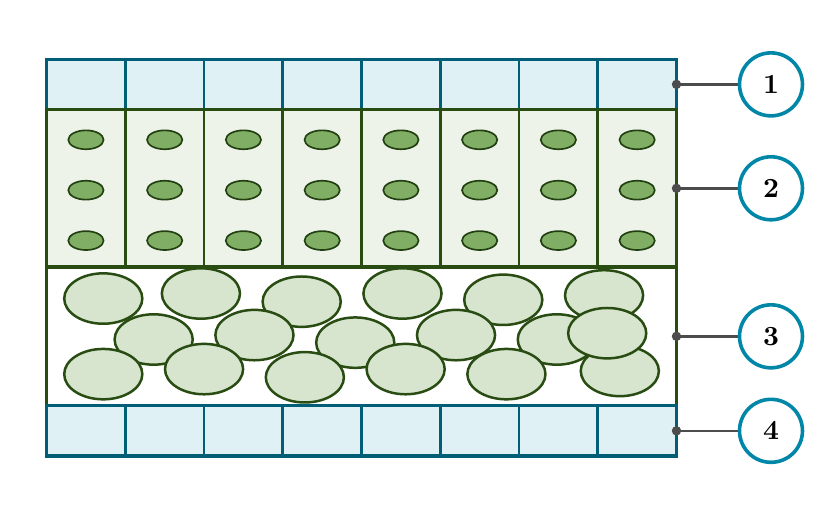
\begin{tikzpicture}[x=0.80cm, y=0.80cm, line cap=round,
    num/.style={circle, draw=cbteal, fill=white, line width=1.3pt,
                inner sep=2pt, minimum size=8mm, font=\bfseries}]

  % ---- upper epidermis: a flat row of bricks -------------------------------
  \fill[cbteal!12] (0,7.0) rectangle (10,7.8);
  \draw[line width=1.2pt, cbteal!70!black] (0,7.0) rectangle (10,7.8);
  \foreach \x in {1.25,2.5,...,8.75}{
    \draw[line width=1pt, cbteal!70!black] (\x,7.0) -- (\x,7.8);}

  % ---- palisade layer: tall columns packed with chloroplasts ---------------
  \fill[cbgreen!10] (0,4.5) rectangle (10,7.0);
  \draw[line width=1.2pt, cbgreen!55!black] (0,4.5) rectangle (10,7.0);
  \foreach \x in {1.25,2.5,...,8.75}{
    \draw[line width=1pt, cbgreen!55!black] (\x,4.5) -- (\x,7.0);}
  \foreach \x in {0.625,1.875,...,9.375}{
    \foreach \y in {4.92,5.72,6.52}{
      \fill[cbgreen!70] (\x,\y) ellipse (0.28 and 0.15);
      \draw[line width=0.6pt, cbgreen!45!black] (\x,\y) ellipse (0.28 and 0.15);}}

  % ---- spongy layer: loose round cells with air gaps between them ----------
  % Every centre is kept at or below x = 9.1 so that no cell (rx = 0.62) bleeds
  % past the right border of the band, which is also where the leader lands.
  \fill[white] (0,2.3) rectangle (10,4.5);
  \draw[line width=1.2pt, cbgreen!55!black] (0,2.3) rectangle (10,4.5);
  \foreach \x/\y in {0.9/4.0, 2.45/4.08, 4.05/3.95, 5.65/4.08, 7.25/3.98, 8.85/4.05,
                     1.7/3.35, 3.3/3.42, 4.9/3.3, 6.5/3.42, 8.1/3.35, 9.1/2.85,
                     0.9/2.8, 2.5/2.88, 4.1/2.75, 5.7/2.88, 7.3/2.8, 8.9/3.45}{
    \fill[cbgreen!22] (\x,\y) ellipse (0.62 and 0.4);
    \draw[line width=0.9pt, cbgreen!55!black] (\x,\y) ellipse (0.62 and 0.4);}

  % ---- lower epidermis: a flat row of bricks -------------------------------
  \fill[cbteal!12] (0,1.5) rectangle (10,2.3);
  \draw[line width=1.2pt, cbteal!70!black] (0,1.5) rectangle (10,2.3);
  \foreach \x in {1.25,2.5,...,8.75}{
    \draw[line width=1pt, cbteal!70!black] (\x,1.5) -- (\x,2.3);}

  % ---- leader lines, each ending in a dot on its own band ------------------
  \foreach \y/\n in {7.4/1, 5.75/2, 3.4/3, 1.9/4}{
    \fill[black!70] (10,\y) circle (0.075);
    \draw[line width=0.9pt, black!70] (10,\y) -- (11.1,\y);
    \node[num] at (11.5,\y) {\n};}

  \path (-0.3,1.0) rectangle (12.1,8.3);
\end{tikzpicture}
\end{center}

\vspace{4pt}
\noindent
\begin{tabularx}{\textwidth}{|c|p{4.6cm}|X|}
  \hline
  \textbf{No.} & \textbf{Name of the tissue} & \textbf{Its job} \\
  \hline
  1 \rule[-1.0em]{0pt}{2.0em} & & \\ \hline
  2 \rule[-1.0em]{0pt}{2.0em} & & \\ \hline
  3 \rule[-1.0em]{0pt}{2.0em} & & \\ \hline
  4 \rule[-1.0em]{0pt}{2.0em} & & \\ \hline
\end{tabularx}
\end{minipage}

\qhead{C5}{Answer in full sentences}

\begin{wordhelp}[Word help --- one word, two completely different meanings]
  {\renewcommand{\arraystretch}{1.15}%
  \begin{tabularx}{\linewidth}{@{}l@{\hspace{1.4em}}X@{}}
    \eng{a tissue} (everyday)   & a paper handkerchief. You can count them:
                                  \emph{a tissue}, \emph{two tissues}. \\
    \eng{tissue} (science)      & a group of similar cells. You do \textbf{not} count
                                  it: \emph{muscle tissue}, not \emph{a muscle
                                  tissue}. \\
  \end{tabularx}}
\end{wordhelp}

% The "finish this sentence: a tissue is similar cells, but an organ is..."
% question used to be first here. It asked students to restate the orange box
% at the top of Section C, and C2's two follow-up lines already make them
% write that contrast about a real leaf. Cut rather than shortened.
\begin{enumerate}[label=\arabic*., itemsep=11pt]

  \item Write \textbf{two sentences of your own}. In the first, use \emph{tissue} with
        its everyday meaning. In the second, use \emph{tissue} with its scientific
        meaning.
        \wlines{3}

  \item A jellyfish has no heart, no lungs and no brain. Which level of the ladder can
        a living thing manage without? Explain your answer.
        \wlines{2}

\end{enumerate}

% ===========================================================================
% ANSWER KEY (teacher copy only)
% ===========================================================================
\ifkey
\newpage
\hwsection[cbred]{Answer Key --- Teacher Copy}

% The key is for an adult at a desk, not a 12-year-old writing on it.
\linespread{1.0}\selectfont
\setlist[enumerate]{itemsep=2pt, topsep=3pt, leftmargin=*}
\setlist[itemize]{itemsep=2pt, topsep=3pt, leftmargin=*}

\qhead[cbred]{A1}{Hunt the pairs}
\noindent (a) $36 = 1\times36,\ 2\times18,\ 3\times12,\ 4\times9,\ 6\times6$.
Factors: 1, 2, 3, 4, 6, 9, 12, 18, 36. \\
(b) $54 = 1\times54,\ 2\times27,\ 3\times18,\ 6\times9$.
Factors: 1, 2, 3, 6, 9, 18, 27, 54. \\
(c) 1, 2, 3, 6, 9, 18 \\
(d) \textbf{18}

\smallskip
\noindent{\small $6 \times 6$ is the one people miss, because it is the same number
twice --- and it is why 36 has an odd number of factors. Worth a sentence at the board
if several students list eight factors instead of nine.}

\qhead[cbred]{A2}{Divide to decide}
\noindent
% 3.4cm columns pushed the "no" after "132 div 8 = 16 r 4" onto a second line.
\begin{tabularx}{\linewidth}{@{}p{4.1cm}p{4.1cm}p{4.1cm}X@{}}
  $96 \div 6 = 16$ \ \textbf{yes} & $96 \div 7 = 13$ r 5 \ no &
  $84 \div 4 = 21$ \ \textbf{yes} & $84 \div 5 = 16$ r 4 \ no \\
  $105 \div 7 = 15$ \ \textbf{yes} & $132 \div 8 = 16$ r 4 \ no &
  $156 \div 12 = 13$ \ \textbf{yes} & $210 \div 6 = 35$ \ \textbf{yes} \\
\end{tabularx}

\smallskip
\noindent{\small Five ticks and three crosses. The one to watch is $132 \div 8$: a
student who has learned ``even numbers divide by 8'' ticks it without dividing. Make
them show the remainder. $156 \div 12$ is the hardest division on the page --- if it is
the only one they get wrong, that is an arithmetic problem, not a factors problem.}

\qhead[cbred]{A3}{Say it, then write it}
\begin{enumerate}[label=\arabic*., itemsep=2pt]
  \item $96 \div 8 = 12$
  \item $72 \div 9 = 8$
  \item HCF$(20,30) = 10$. Factors of 20: 1, 2, 4, 5, 10, 20. Of 30: 1, 2, 3, 5, 6, 10,
        15, 30. Common: 1, 2, 5, 10.
  \item $81 \div 6 = 13$ r 3, so \textbf{no} --- 6 does not divide into 81 exactly.
\end{enumerate}
\noindent{\small Question 4 is the one that tests whether ``exactly'' has landed. An
answer of ``13.5'' is not wrong arithmetic but it is the wrong question: at this stage
we want the remainder, because the remainder is what decides whether it is a factor.}

\qhead[cbred]{A4}{What the HCF is actually for}
\noindent
\begin{tabularx}{\linewidth}{@{}p{2.6cm}p{1.8cm}p{3.2cm}p{3.4cm}X@{}}
  $18/24$ & HCF 6  & $18 \div 6 = 3$   & $24 \div 6 = 4$   & $\mathbf{3/4}$ \\
  $30/45$ & HCF 15 & $30 \div 15 = 2$  & $45 \div 15 = 3$  & $\mathbf{2/3}$ \\
  $48/60$ & HCF 12 & $48 \div 12 = 4$  & $60 \div 12 = 5$  & $\mathbf{4/5}$ \\
\end{tabularx}

\smallskip
\noindent{\small The predictable error is using \emph{a} common factor rather than the
\emph{highest} one --- dividing $18/24$ by 2 to get $9/12$ and stopping. That is not
wrong, it is unfinished, and the fix is to say so in those words. Six divisions live in
this question; if a student's HCF is right and the fraction is wrong, the failure is
division, not factors.}

\qhead[cbred]{A5}{Two answers that surprise people}
\noindent (a) \textbf{1} --- not ``none''. 9 and 10 are consecutive, so 1 is the only
number in both lists. \\
(b) \textbf{7} --- not 1. 7 divides into 42, so the HCF is just the smaller number.

\smallskip
\noindent (c) Any sentence saying that \textbf{1 is a factor of every number}, so every
pair of numbers has at least one common factor.

\smallskip
\noindent{\small These are the two mirror-image errors from the lesson, and they are on
the page together on purpose. Expect ``none'' for (a) and ``1'' for (b) from the same
students. Mark (c) strictly: it must name 1, not just say ``it is never true''.}

\qhead[cbred]{A6}{Word problems}
\begin{enumerate}[label=\arabic*., itemsep=2pt]
  \item HCF$(42,56) = 14$, so \textbf{14 bracelets}, each with $42 \div 14 = 3$ red
        beads and $56 \div 14 = 4$ blue beads. (Factors of 42: 1, 2, 3, 6, 7, 14, 21,
        42. Of 56: 1, 2, 4, 7, 8, 14, 28, 56.)
  \item $45/60$. HCF$(45,60) = 15$, so $45 \div 15 = 3$ and $60 \div 15 = 4$:
        \textbf{3/4}.
\end{enumerate}
\noindent{\small In problem 1, students who answer ``14'' have done the maths but not
the question --- the beads per bracelet are two more divisions and they are what the
HCF was for. Problem 2 is the same method as A4 wearing a story; if a student can do A4
and not this, the gap is reading, not arithmetic.}

\qhead[cbred]{B1}{The factor hunt}
\noindent
\begin{tabularx}{\linewidth}{@{}lX@{}}
  \textbf{1260} & yes: 2, 3, 4, 5, 6, 9, 10 \quad no: 8, 11 \\
  \textbf{3465} & yes: 3, 5, 9, 11 \quad no: 2, 4, 6, 8, 10 \\
  \textbf{2088} & yes: 2, 3, 4, 6, 8, 9 \quad no: 5, 10, 11 \\
  \textbf{4510} & yes: 2, 5, 10, 11 \quad no: 3, 4, 6, 8, 9 \\
  \textbf{5832} & yes: 2, 3, 4, 6, 8, 9 \quad no: 5, 10, 11 \\
\end{tabularx}

\smallskip
\noindent Digit sums: 1260 gives 9, 3465 gives 18, 2088 gives 18, 4510 gives 10,
5832 gives 18. Last three digits for the test for 8: 260 (no), 465 (no), 088 (yes,
$88 \div 8 = 11$), 510 (no), 832 (yes, $832 \div 8 = 104$).
Groups for the test for 11: 1260 gives 7 and 2 (difference 5, no); 3465 gives 9 and 9
(difference 0, \textbf{yes}); 2088 gives 10 and 8 (difference 2, no); 4510 gives 5 and
5 (difference 0, \textbf{yes}); 5832 gives 8 and 10 (difference 2, no).

\smallskip
\noindent{\small The row worth marking carefully is \textbf{1260}: it divides by 4 but
\emph{not} by 8, which kills ``divisible by 4 means divisible by 8''. The other trap is
\textbf{4510} --- it is even, so students tick 6 without checking the digit sum, which
is 10 and fails the test for 3. Both errors are conceptual, not careless.}

\qhead[cbred]{B2}{Now prove it}
\noindent (a) $315$ \quad (b) $140$ \quad (c) $315$ \quad (d) $261$ \quad (e) $902$
\quad (f) $972$

\smallskip
\noindent (g) \textbf{(a) and (c)} --- both come to 315.

\smallskip
\noindent{\small This question is the division practice of the packet and it is where
weak arithmetic will show. (c) $3465 \div 11$ is the hardest; (e) $4510 \div 5$ is the
easiest and is there so everybody finishes something. Part (g) is not decoration: it
makes them look back at their own six answers, which is the check they never do
voluntarily.}

\qhead[cbred]{B3}{The missing digit}
\begin{enumerate}[label=\arabic*., itemsep=3pt]
  \item $5 + 2 = 7$. The digit sum must reach 9, 12 or 15, so the digit is
        \textbf{2, 5 or 8} (giving 522, 525, 528).
  \item $7 + 4 + 1 = 12$. The next multiple of 9 is 18, and $18 - 12 = 6$, so the digit
        is \textbf{6} and the number is 7416. (Only one answer: the multiple after 18
        is 27, which would need a digit of 15.)
  \item Groups are $\square + 3$ and $6 + 0 = 6$. For a difference of 0 we need
        $\square + 3 = 6$, so the digit is \textbf{3} and the number is 3630.
        ($3630 \div 11 = 330$.)
\end{enumerate}
\noindent{\small Question 1 is the one that tests whether they believe an answer can be
a set rather than a number --- most will find one digit and stop. Ask ``are you sure
that is the only one?'' rather than marking it wrong.}

\qhead[cbred]{B4}{Word problems}
\begin{enumerate}[label=\arabic*., itemsep=2pt]
  \item The last three digits are 368, and $368 \div 8 = 46$, so 4176 divides by 8:
        \textbf{yes}, with none left over. $4176 \div 8 = \mathbf{522}$ stickers each.
  \item 2464 is even, so it makes $2464 \div 2 = 1232$ pairs. For 11: the groups are
        $2 + 6 = 8$ and $4 + 4 = 8$, a difference of 0, so 2464 divides by 11 --- and
        so does 1232, giving $1232 \div 11 = \mathbf{112}$ drawers.
        Mr Bowen has two feet.
\end{enumerate}
\noindent{\small Problem 2 is the deadpan one. Read it completely straight and do not
explain the joke; the maths is correct and that is the whole point. It is also a
two-step division, which is harder than it looks --- a student who divides 2464 by 11
directly gets 224, which is the number of \emph{socks} per drawer, not the number of
drawers. Both routes are defensible if they say which they took.}

\qhead[cbred]{B5}{Now you write the question}
\noindent No single right answer. Check, in this order:
\begin{enumerate}[label=\arabic*., itemsep=2pt]
  \item \textbf{Is it a sharing story?} Something split into 8 equal groups, or packed
        8 to a box. A story where 8 things are bought is a multiplication, not this.
  \item \textbf{Does it say ``equally'' or ``with nothing left over''?} Without that,
        the question does not have a single answer.
  \item \textbf{Full sentences, ending in a question?}
  \item \textbf{Does their own answer come out as 546?}
\end{enumerate}
\noindent (b) The last three digits are \textbf{368}, and $368 \div 8 = 46$, so 4368
divides by 8.

\smallskip
\noindent{\small One that works for (a): ``A factory packs 4368 eggs into boxes. Each
box holds 8 eggs, and every box is full. How many boxes do they fill?'' \\
Part (b) is the one worth marking hardest: it is the difference between knowing the
test and having memorised an answer. A student who writes ``because I divided it'' has
answered the opposite of the question that was asked.}

\qhead[cbred]{C1}{Match the word to its meaning}
\noindent 1--B \quad 2--C \quad 3--D \quad 4--A \quad 5--F \quad 6--E

\qhead[cbred]{C2}{Which level is it?}
\noindent
\begin{tabularx}{\linewidth}{@{}p{4.4cm}p{3.4cm}p{4.4cm}X@{}}
  a red blood cell   & cell         & the digestive system & organ system \\
  a leaf             & \textbf{ORGAN}  & onion epidermis   & tissue \\
  the palisade layer & \textbf{TISSUE} & Mr Bowen          & organism \\
  the heart          & organ        & a root hair cell     & cell \\
\end{tabularx}

\smallskip
\noindent A leaf is an \textbf{organ} because it is made of four \emph{different}
tissues. The palisade layer is a \textbf{tissue} because it is made of cells that are
all \emph{similar} and all do one job.

\smallskip
\noindent{\small These two are the deliberate traps and they fail in opposite
directions: a leaf looks like one flat thing so it gets called a tissue, and the
palisade layer has an important-sounding name so it gets called an organ. If the class
splits on these two, do not mark it --- put the leaf cross-section back on the board
and count the four layers out loud.}

\qhead[cbred]{C3}{Climb the ladder}
\noindent Cell: a ciliated cell \ $\rightarrow$ \ Tissue: ciliated epithelium \
$\rightarrow$ \ Organ: a lung \ $\rightarrow$ \ Organ system: the breathing system \
$\rightarrow$ \ Organism: a human (accept ``me'', ``Mr Bowen'', ``a person'').

\smallskip
\noindent{\small The rung most often wrong is the organ: students write ``the lungs''
or jump straight to ``the breathing system''. One lung is the organ; the pair plus the
windpipe and the nose is the system. Accept ``a lung'' or ``the lungs'' but not
``breathing''.}

\qhead[cbred]{C4}{Label the leaf}
\noindent
\begin{tabularx}{\linewidth}{@{}p{0.8cm}p{4.4cm}X@{}}
  1 & upper epidermis & a flat protective skin over the top of the leaf \\
  2 & palisade layer  & tall cells packed with chloroplasts, where most
                        photosynthesis happens \\
  3 & spongy layer    & loose round cells with air gaps, letting gases move through
                        the leaf \\
  4 & lower epidermis & the protective skin underneath \\
\end{tabularx}

\smallskip
\noindent{\small 1 and 4 are the same tissue in two places, so accept ``epidermis'' for
both only if the student writes \emph{upper} and \emph{lower}. The layer most often
mislabelled is 3: it gets called ``the air layer'' or ``the gaps''. The gaps are the
point of it, but the tissue is the cells around them. \\
Coming back to C2: this diagram is the answer to why a leaf is an organ --- four
different tissues, one structure.}

\qhead[cbred]{C5}{Answer in full sentences}
\begin{enumerate}[label=\arabic*., itemsep=3pt]
  \item Everyday: ``Mr Bowen sneezed, so he took a tissue out of the box.''
        Scientific: ``The wall of the stomach contains muscle tissue.''
        Mark the \textbf{sentence} --- capital letter, full stop, and the countable
        versus uncountable difference actually showing.
  \item The \textbf{organ system} level, and arguably the organ level too. A jellyfish
        has cells and tissues but no heart, lungs or brain, so a living thing can exist
        without organ systems. The bottom two rungs are the ones every organism has.
\end{enumerate}
\noindent{\small Question 1 is the real English work in this section and is worth more
of your marking time than the rest of C put together. The commonest failure is two
sentences that both use the everyday meaning. Question 2 has no tidy answer and should
be discussed rather than ticked --- accept anything that spots a living thing can
manage without the top rungs.}

\fi

\end{document}
